\chapter{提案}
本章では,SBCを用いたマルチディスプレイシステムにおけるOS仮想化技術を用いた仮想化と,コンテナ技術を用いたSBCマルチディスプレイシステムのフレーム処理並列化について設計・提案する.
本章では,まず3.1節でOS仮想化基盤とコンテナ技術について簡単に説明する.
そして,続く3.2節でOS仮想化基盤を利用したSBCマルチディスプレイシステムのコンテナ仮想化についての設計と実装について述べる.
3.3章では映像ベースのアプリケーションをコンテナ仮想化することによって生じる問題と,その解決法について述べる.
3.4章では,本研究の中心部分となるヘッドノード内でのフレーム処理の改良について,その設計指針を述べ,
具体的な実装について記す.

\section{OS仮想化基盤とコンテナ技術}
OS仮想化基盤には,代表的なものとしてDocker \cite{docker}が挙げられる.
Dockerは,Docker社が開発しているプラットフォームであり,Dockerを用いることで,マシン内にコンテナと呼ばれる仮想環境を作成,実行することができる.

DockerをはじめとしたOS仮想化と比較されるのが,ハイパーバイザ型仮想化である.ハイパーバイザ型仮想化は,ホストマシンとなる物理マシン上でハイパーバイザと呼ばれる仮想マシン (VM) を作成および実行するソフトウェアを動作させ,それを通じて仮想化環境を制御するものである.
ハイパーバイザ型仮想化は,移植面で汎用性が高いことが長所である.一方で,ホストOSを介して仮想環境の制御を行うため,制御のオーバーヘッドが大きく処理が低速になるという欠点を持つ.
それに対して,コンテナを用いたOS仮想化技術では仮想化環境 (コンテナ) はホストマシンのOSを使用する.そのため,コンテナは軽量に動作し仮想環境の起動や終了も小さいオーバーヘッドで行えるのが特徴である.

ハイパーバイザ型仮想化とコンテナ技術を用いたOS化の概要を図xxxに示す.

\begin{figure}[H]
    \hspace*{\fill}
    
\includegraphics[width=\linewidth]{./fig/dummy.eps}
    \hspace*{\fill}
    \caption{ハイパーバイザ型仮想化とコンテナを用いたOS仮想化}
\end{figure}

さらに,Dockerを利用することで様々な利点も生まれる.

まず,仮想化環境をコード化して管理する事で,どのような環境の上にでも同一の環境を作成する事ができる点である.
Dockerでは仮想化環境の構築情報をコード化されたファイルとして管理する.
このファイルを保存し配布する事で,特定の環境を再現し,複数のマシン上で全く同一の環境を作り出すことが可能となる.
この機能は,ソフトウェアの開発やテストなど,異なるマシンで同一の環境を作成し,その上でアプリケーションを動作させる必要のある場合などによく利用されている.

また,環境の作成や廃棄が簡単であることも利点の1つである.
複数のサーバを連携させて全体で1台のサーバであるかのように動作させるクラスタを構築する場合も、Dockerイメージがあれば、それを元に複数の環境(コンテナ)を起動できる.
この機能を活用することにより環境を一から作る作業もなくなり、クラスタ構成を構築するのも容易になる.
さらに,Kubernetes \cite{k8s}などのコンテナオーケストレーションシステムを用いてクラスタ環境を管理することも容易になる.



\section{MDのコンテナ化}
前節で紹介したような仮想化技術を用いることで,異なるマシンでもアプリケーションを同一の環境で動作させる事ができる.
この仮想化技術を用いて,2章で先行研究として紹介したSBCを用いたマルチディスプレイシステムを仮想化することを考える.

先行研究では,SBCマルチディスプレイシステムにおいてディスプレイノードにRaspberry Piを使用している.
しかし,2022年2月現在においてはSBCの開発は盛んに行われており,市場には数百種類ものSBCが存在している \cite{hackerbords}.
それらのSBCの間ではアーキテクチャやOS,ディスプレイの描画方法,対応言語などに違いが存在する.
そのため,これらのSBCを用いてマルチディスを構築すると構築の手順や動作に違いが発生する事が考えられる.
そのため,異なるSBCを用いた際に発生するこれらの差異を吸収するため,様々なSBCに対応することができるようなミドルウェアの開発が必要である.
そこで,前節で紹介したコンテナ仮想化技術であるDockerの利用を検討する.

\begin{figure}[H]
    \hspace*{\fill}
    \includegraphics[width=\linewidth]{./fig/md_docker.eps}
    \hspace*{\fill}
    \caption{Dockerを用いた環境構築}
\end{figure}

Dockerを用いた環境構築の概要図を図xxxに示す.
ユーザは,まずヘッドノードもしくはディスプレイノードとして利用するマシンに対してDockerのインストール作業を行う.
次に, Dockerのコマンドを用いてGitHub上のリポジトリからソースコードを取得し,その中に含まれているDockerfileを用いてホストマシン内にコンテナ環境を作成する.ここでDockerfileとはコンテナ環境の構成情報 (OS, パッケージ,ネットワーク設定情報など) を保存したファイルであり,これを用いてコンテナ環境を構築することにより簡単にあらかじめ準備されていた環境を構築する事ができる.
最後に,ホストマシン上に構成したコンテナ環境内でプログラムのビルドを行う事で,そのマシンをヘッドノードもしくはディスプレイノードとして使用する事が可能になる.

\section{コンテナを通したディスプレイの制御}
本節では,コンテナ技術を用いて構築したMDにおける,フレームのディスプレイ時に生じる問題とその対処について説明する.
マシンに接続されたディスプレイに画像を表示する際には,一般にはフレームバッファと呼ばれる領域が使用される.
フレームバッファは/devディレクトリに存在するデバイスファイルである.このファイルにディスプレイに表示するデータを格納することで,OSがディスプレイの画像を描画するという仕組みである.
フレームバッファを用いたディスプレイへの画像表示の概要を図xxxに示す.

\begin{figure}[H]
    \hspace*{\fill}
    
\includegraphics[width=\linewidth]{./fig/dummy.eps}
    \hspace*{\fill}
    \caption{ハイパーバイザ型仮想化とコンテナを用いたOS仮想化}
\end{figure}

Dockerを用いて構築したコンテナ環境の内部からは,ホストマシンのリソースへのアクセスが制限される場合がある.
例えば,デフォルトの状態ではDockerコンテナはDockerコンテナの内部でDocker daemonの起動を行うことができない.
これは、デフォルトではコンテナからホストマシンのデバイスへのアクセスが許されていないためである.
同様に,フレームバッファもDockerコンテナの内部から見ればホストマシンのデバイスファイルであるため,ファイルが操作できずにディスプレイへの画像表示が不可能になっている.この状態を,コンテナはunprivilegedな状態であるという.

対して,privilegedなコンテナはホストマシンの全てのリソースにアクセスする事が可能である.コンテナをpriviledgeな状態で起動するのは,起動時のコマンドで--privilegedコマンドを指定する必要がある.

\section{ヘッドノードでのフレーム処理の改良}
ここまでで,SBCマルチディスプレイシステムをコンテナ基盤上で動作させる事ができた.続いて本節以降では,本研究の提案の中心部分であるヘッドノードでのフレーム処理の改良について述べる.

2章でも説明した通り,先行研究で提案されたマルチディスプレイには高解像度な動画や,高フレームレートな動画をMD上に表示しようとするとヘッドノードでの処理がボトルネックとなり動画表示に遅延が発生するという課題がある.
高解像度な動画はフレームの分割や圧縮にかかる時間が大きくなるため,ヘッドノード内での処理時間が増加し,フレームの表示処理への影響も大きくなる.
また,高フレームレートな動画の場合には,フレーム処理時間の影響により元々のフレームレートを維持たまま動画を表示することが困難になる.
さらに,大規模なMDを構築した際の性能低下も課題点としてあげられる.
先行研究のMDではヘッドノード内でフレーム圧縮を行うスレッドが1つであるため,MDを構成するディスプレイ数が増加するのに伴ってスレッドでの処理負荷が増加する.
その結果,MDの大規模化に伴ってフレーム処理にかかる時間も増加し,動画再生時のフレームレートが低下する.

この問題に対して提案では,ヘッドノードでのフレーム処理を並列化したプロセスとして実装し,ヘッドノード内での処理時間を短縮する.

\subsection*{フレーム処理のコンテナ並列化}
提案手法の実装にはOS仮想化技術を用いたコンテナ技術を使用し,プロセスレベルでの並列化を図ります.
また,処理の並列化に伴うプロセス間での画像フレームの受け渡しについては,高速なプロセス間通信を行える共有メモリを使用することでオーバーヘッドの低減を目指します.

先行研究では,ヘッドノード内の圧縮スレッド内でフレーム切り出し,フレーム分割,フレーム圧縮の3種類の処理が行われている.

フレーム切り出しとフレーム分割はディスプレイ数に関わらず1フレームに対して1回の処理のみが行われるが,フレームの圧縮はマルチディスプレイを構成するディスプレイ数に応じて処理回数が変化するため,この部分がシステムのボトルネックとなる.
このボトルネックを解消するために,圧縮処理をヘッドノード内で並列化して行い,全体での処理時間を短縮する.

\begin{figure}[H]
    \hspace*{\fill}
    \includegraphics[width=\linewidth]{./fig/process_parallelization.eps}
    \hspace*{\fill}
    \caption{フレーム処理の並列化}
\end{figure}


提案手法では,ヘッドノード内で行われる処理それぞれを単一のコンテナに分割し,画像フレームの切り出し・分割を行う分割コンテナ,フレームの圧縮処理を行う圧縮コンテナ,そしてディスプレイノードとの同期用通信を行う同期制御コンテナの3種類のコンテナとして実装する.
圧縮コンテナは構成ディスプレイと同じ数だけ用意し,ヘッドノード内で並列化してフレームの圧縮処理を行う.



ヘッドノード内でのコンテナを用いたフレーム処理の並列化について書く
メインコンテナ,圧縮コンテナの実装や動作などについて図やフローチャートを用いて解説する

\subsection*{コンテナ間でのフレーム受け渡し処理}

処理の並列化を目的としてフレームの分割を行うコンテナと圧縮を行うコンテナを分けたことにより,ヘッドノード内のコンテナ間で画像フレームの受け渡しを行う必要が生じる.
この処理によるオーバヘッドを抑えるために,高速なプロセス通信が可能な共有メモリ (System V IPC) \cite{kerrisk2010linux,linux_kernel}を使用する.

以下,共有メモリ (System V IPC) について簡単に説明する.
IPCとはプロセス間通信 (InterProcess Communication) の略であり,ユーザモードプロセスから

\begin{itemize}
    \item セマフォを利用した他のプロセスとの同期
    \item 他のプロセスとの間でのメッセージ送受信
    \item 他のプロセスとのメモリ領域の共有
\end{itemize}

System V IPCは,現在ではLinuxを含むほとんどのUNIXシステムで使用できるようになっている.
IPCのデータ構造は,プロセスがIPC資源 (セマフォ,メッセージキュー,共有メモリリージョン) を要求した際に動的に作成される.
IPC資源を要求したプロセスが獲得した資源を明示的に解放しない限りIPC資源はメモリ上に残り続け,他のどのプロセスからでも使用できる状態になる.
各資源は,ファイルシステムツリーにおけるファイルのパス名に相当する32ビットのIPCキーによって識別される.また,各IPC資源は32ビットのIPC識別子を持つ.IPC資源はカーネルによって決定されるが,IPCキーは自由に決める事が可能である.複数のプロセスがIPC資源を利用する際には,IPC識別子が利用される.
本研究の実装ではSystem V IPCを利用して共有メモリ領域を獲得し,異なるプロセス間でのデータ共有を高速に行うことを目的とする.

続いて,IPC資源の利用方法について説明する.
System V IPCを用いて共有メモリ領域を獲得するのは,shmget()関数を用いる.
shmget()関数は引数として渡されたIPCに対応するIPC識別子を取得し,そのIPC識別子を利用することでプロセスが共有メモリ領域にアクセスすることができるようになる.
別々のプロセスから同一のIPC資源を共有するための方法は2通り存在する.
1つはプロセス間であらかじめ固定のIPCキーを決定しておく方法である.
この方法は単純であるため,多くのプロセスが関連する複雑なアプリケーションで利用してもうまく動作する.しかし,全く関係ないプロセスが偶然同じIPCキーを使用してしまう可能性がある.
もう1つは,一方のプロセスでIPCキーにIPC\_PRIVATEを指定する方法である.この方法では新規のIPC資源が割り当てられ, そのIPC識別子によってアプリケーション内の他のプロセスとの通信を行うため,他のプロセスから誤ってIPC資源を利用されてしまうことを防げる.

以上の方式を検討した結果,本研究ではIPC資源が複数のプロセスから参照されるため,前者の手法を採用して実装を行った.

\subsection*{IPC共有メモリ}

IPC共有メモリでは,共有するデータ構造をIPC共有メモリリージョンに配置することにより,複数のプロセスから共有データ構造にアクセスする事ができる.
IPC共有メモリは,まずプロセス1が共有メモリと識別子を作成し,その後にプロセス2が同じ識別子を用いて共有メモリをプロセス2のアドレス空間にアタッチすることで使用することができる.
この手続きを行うことで,共有メモリを介して画像フレームなどを渡すことが可能になる.

\begin{figure}[H]
    \hspace*{\fill}
    
\includegraphics[width=\linewidth]{./fig/shared_memory.eps}
    \hspace*{\fill}
    \caption{共有メモリの使用例}
\end{figure}

\begin{figure}[H]
    \hspace*{\fill}
    \includegraphics[width=\linewidth]{./fig/shared_memory2.eps}
    \hspace*{\fill}
    \caption{共有メモリの使用例2}
\end{figure}

実際の処理では,まず分割コンテナがフレームの切り出しと分割を行った後,圧縮コンテナとの間に作成された共有メモリにフレームデータを格納する.
圧縮コンテナは共有メモリに格納されたフレームを取得し,圧縮処理を行う.

共有メモリはヘッドノードの中に1つのみを作成し,その中でそれぞれの圧縮コンテナに対してメモリ領域を割り当てるという方式を取る.
また,共有メモリにはフレーム切り出しの際に使われるOpenCVのMat形式からキャラクタ型の配列に変換してフレームデータを格納する.


図3.7に提案手法を用いて構築したMDの動作フローを示す.
ヘッドノードでは分割コンテナ,圧縮コンテナ,同期制御コンテナの3種類のコンテナが動作している.
まず画像フレームが分割コンテナによって分割され,バッファを通じて圧縮コンテナへ渡される.
圧縮コンテナはこのフレームに対してJPEG圧縮処理を行い,それぞれが接続しているディスプレイノードへと送信する.

ディスプレイノードではフレームを受信したのち展開処理を行い,フレームバッファに書き込むことでディスプレイへ画像を表示する.

ヘッドノードで操作している同期制御コンテナはディスプレイノードからの同期メッセージを受け取り,フレーム表示命令を送信するとともに,圧縮コンテナ内で行われているフレーム圧縮のパラメータを制御することでフレームレートを一定に保つ役割を持つ.

\begin{figure}[H]
    \hspace*{\fill}
    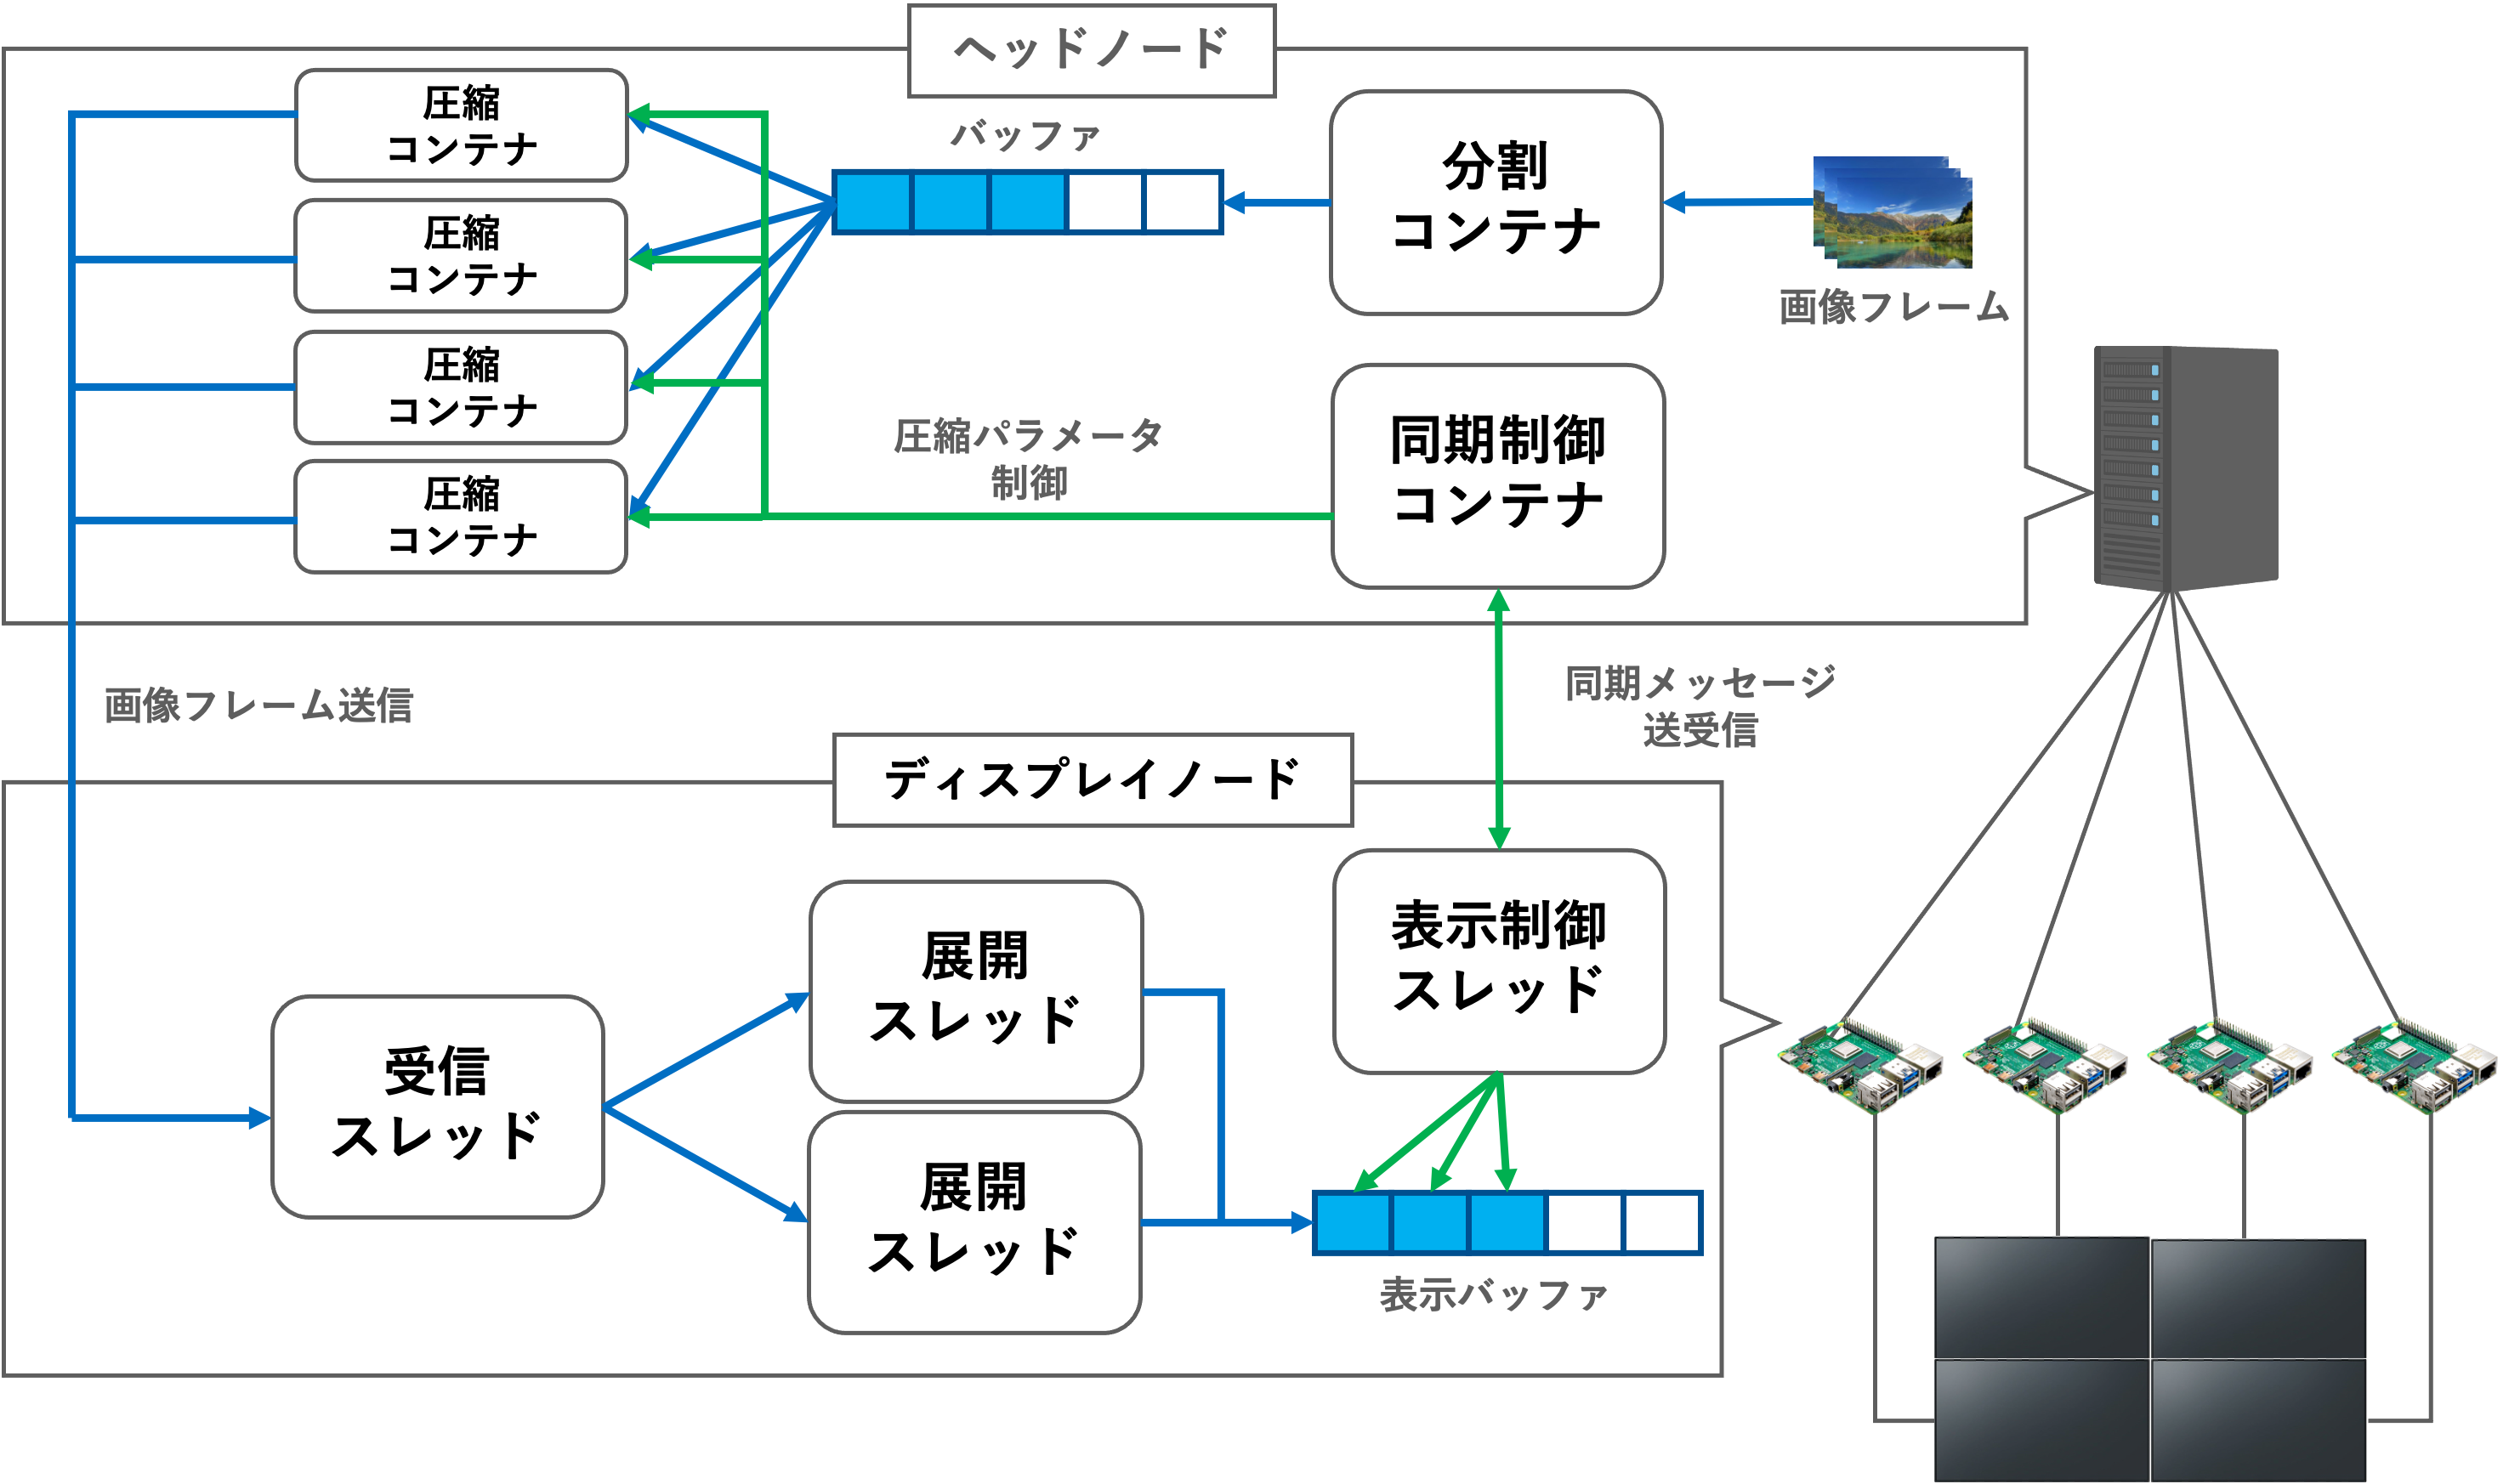
\includegraphics[width=\linewidth]{./fig/system_flow.eps}
    \hspace*{\fill}
    \caption{提案手法を用いたMDの動作フロー}
\end{figure}
